\RequirePackage{atbegshi}
\documentclass[compress,dvipsnames, aspectratio=169]{beamer} % aspectratio=169
%\usepackage[svgnames]{xcolor}

%	%	%	%	%	%	%	%	%	%	%	%	%	%	%
% 						MY PACKAGES 
%	%	%	%	%	%	%	%	%	%	%	%	%	%	%
\usepackage{graphicx}				% Use pdf, png, jpg, or eps with pdflatex; use eps in DVI mode

\usepackage[export]{adjustbox}

\usepackage{amssymb}
\usepackage{amsmath}	
%\usepackage{tipx}
%\usepackage{tikz}
%\usetikzlibrary{arrows,shapes,decorations.pathmorphing,backgrounds,positioning,fit,petri}
\usepackage{rotating}
\usepackage{scalerel} % for inline images
\usepackage{import}
%\usepackage{times}
\usepackage{array}
\usepackage{tabularx}
%\usepackage{booktabs}
\usepackage{textcomp}
\usepackage{caption}
\usepackage{float}
%\usepackage{setspace} 			% \doublespacing \singlespacing \onehalfspacing	%doble espacio
%\label{x:y}													%ocupar para autoref.
%\autoref{x:y}												%ocupar para autoref.
%\usepackage{nopageno}			%desactivar para p�ginas
\usepackage{pifont}
\usepackage{color,xcolor,ucs}
%\usepackage{marvosym} %faces

\usepackage{hyperref}
\usepackage{multirow}

\usepackage{listings}
\usepackage{color}
\definecolor{dkgreen}{rgb}{0,0.6,0}
\definecolor{gray}{rgb}{0.5,0.5,0.5}
\definecolor{mauve}{rgb}{0.58,0,0.82}
\lstset{ %
  language=R,                     % the language of the code
  basicstyle=\TINY,      			% the size of the fonts that are used for the code
  numbers=left,                   % where to put the line-numbers
  numberstyle=\tiny\color{gray},  % the style that is used for the line-numbers
  stepnumber=1,                   % the step between two line-numbers. If it's 1, each line
                                  % will be numbered
  numbersep=5pt,                  % how far the line-numbers are from the code
  backgroundcolor=\color{white},  % choose the background color. You must add \usepackage{color}
  showspaces=false,               % show spaces adding particular underscores
  showstringspaces=false,         % underline spaces within strings
  showtabs=false,                 % show tabs within strings adding particular underscores
  frame=single,                   % adds a frame around the code
  rulecolor=\color{black},        % if not set, the frame-color may be changed on line-breaks within not-black text (e.g. commens (green here))
  tabsize=1,                      % sets default tabsize to 2 spaces
  captionpos=b,                   % sets the caption-position to bottom
  breaklines=true,                % sets automatic line breaking
  breakatwhitespace=false,        % sets if automatic breaks should only happen at whitespace
  title=\lstname,                 % show the filename of files included with \lstinputlisting;
                                  % also try caption instead of title
  keywordstyle=\color{blue},      % keyword style
  commentstyle=\color{dkgreen},   % comment style
  stringstyle=\color{mauve},      % string literal style
  escapeinside={\%*}{*)},         % if you want to add a comment within your code
  morekeywords={*,...}            % if you want to add more keywords to the set
} 

%	%	%	%	%	%	%	%	%	%	%	%	%	%	%
% 					PACKAGE CUSTOMIZATION
%	%	%	%	%	%	%	%	%	%	%	%	%	%	%

% GENERAL CUSTOMIZATION
\usepackage[math]{iwona}% font
\usetheme{Singapore}	% template I should use
%\usetheme{Szeged}	% alternative template
\usecolortheme{rose}	% color template
\makeatletter			% to show subsection/section title (1/3)
\beamer@theme@subsectiontrue % to show subsection/section title (2/3)
\makeatother			% to show subsection/section title (3/3)



% THIS BELOW IS TO MAKE NAVIGATION DOTS MARKED DURING PRESENTATION
\makeatletter
\def\slideentry#1#2#3#4#5#6{%
  %section number, subsection number, slide number, first/last frame, page number, part number
  \ifnum#6=\c@part\ifnum#2>0\ifnum#3>0%
    \ifbeamer@compress%
      \advance\beamer@xpos by1\relax%
    \else%
      \beamer@xpos=#3\relax%
      \beamer@ypos=#2\relax%
    \fi%
  \hbox to 0pt{%
    \beamer@tempdim=-\beamer@vboxoffset%
    \advance\beamer@tempdim by-\beamer@boxsize%
    \multiply\beamer@tempdim by\beamer@ypos%
    \advance\beamer@tempdim by -.05cm%
    \raise\beamer@tempdim\hbox{%
      \beamer@tempdim=\beamer@boxsize%
      \multiply\beamer@tempdim by\beamer@xpos%
      \advance\beamer@tempdim by -\beamer@boxsize%
      \advance\beamer@tempdim by 1pt%
      \kern\beamer@tempdim
      \global\beamer@section@min@dim\beamer@tempdim
      \hbox{\beamer@link(#4){%
          \usebeamerfont{mini frame}%
          \ifnum\c@section>#1%
            %\usebeamercolor[fg]{mini frame}%
            %\usebeamertemplate{mini frame}%
            \usebeamercolor{mini frame}%
            \usebeamertemplate{mini frame in other subsection}%
          \else%
            \ifnum\c@section=#1%
              \ifnum\c@subsection>#2%
                \usebeamercolor[fg]{mini frame}%
                \usebeamertemplate{mini frame}%
              \else%
                \ifnum\c@subsection=#2%
                  \usebeamercolor[fg]{mini frame}%
                  \ifnum\c@subsectionslide<#3%
                    \usebeamertemplate{mini frame in current subsection}%
                  \else%
                    \usebeamertemplate{mini frame}%
                  \fi%
                \else%
                  \usebeamercolor{mini frame}%
                  \usebeamertemplate{mini frame in other subsection}%
                \fi%
              \fi%
            \else%
              \usebeamercolor{mini frame}%
              \usebeamertemplate{mini frame in other subsection}%
            \fi%
          \fi%
        }}}\hskip-10cm plus 1fil%
  }\fi\fi%
  \else%
  \fakeslideentry{#1}{#2}{#3}{#4}{#5}{#6}%
  \fi\ignorespaces
  }
\makeatother

%	%	%	%	%	%	%	%	%	%	%	%	%	%	%
% 			To show the TITLE at the Bottom of each slide
%	%	%	%	%	%	%	%	%	%	%	%	%	%	%

\beamertemplatenavigationsymbolsempty 
\makeatletter
\setbeamertemplate{footline}
{
\leavevmode%
\hbox{%
\begin{beamercolorbox}[wd=1\paperwidth,ht=2.25ex,dp=2ex,center]{title in head/foot}%
\usebeamerfont{title in head/foot}\insertshorttitle
\end{beamercolorbox}%
\begin{beamercolorbox}[wd=1
\paperwidth,ht=2.25ex,dp=2ex,center]{date in head/foot}%
\end{beamercolorbox}}%
}
\makeatother



% to switch off navigation bullets
%% using \miniframeson or \miniframesoff
\makeatletter
\let\beamer@writeslidentry@miniframeson=\beamer@writeslidentry
\def\beamer@writeslidentry@miniframesoff{%
  \expandafter\beamer@ifempty\expandafter{\beamer@framestartpage}{}% does not happen normally
  {%else
    % removed \addtocontents commands
    \clearpage\beamer@notesactions%
  }
}
\newcommand*{\miniframeson}{\let\beamer@writeslidentry=\beamer@writeslidentry@miniframeson}
\newcommand*{\miniframesoff}{\let\beamer@writeslidentry=\beamer@writeslidentry@miniframesoff}
\makeatother

% Image full size: use 
%%\begin{frame}
  %%\fullsizegraphic{monogram.jpg}
%%\end{frame}
\newcommand<>{\fullsizegraphic}[1]{
  \begin{textblock*}{0cm}(-1cm,-3.78cm)
  \includegraphics[width=\paperwidth]{#1}
  \end{textblock*}
}


% hyperlinks
\hypersetup{colorlinks,
            urlcolor=[rgb]{0.01, 0.28, 1.0},
            linkcolor=[rgb]{0.01, 0.28, 1.0}}








%	%	%	%	%	%	%	%	%	%	%	%	%	%	%
% 					DOCUMENT ID
%	%	%	%	%	%	%	%	%	%	%	%	%	%	%

\title{Interview with Turku University}
\author{Hector Bahamonde $\bullet$ Assistant Professor $\bullet$ O'Higgins University (Chile)}
\date{June 22nd, 2021}

%to to see shadows of previous blocks
%\setbeamercovered{dynamic}


\begin{document}



%	%	%	%	%	%	%	%	%	%	%	%	%	%	%
% 					CONTENT
%	%	%	%	%	%	%	%	%	%	%	%	%	%	%

%% title frame

\begin{frame}[label = cover]
\titlepage
\end{frame}



\section{Introduction}

%section{Outline}
\subsection{Introduction}

\miniframesoff
\begin{frame}\frametitle{The Order of the Day}
In this presentation I will...
\begin{enumerate}
	\item Briefly describe my {\bf profile}.
	\item Quickly mention three of my most important {\bf publications}.
	\item Explain my 3-year {\bf research plans} at Turku.
	\item Enumerate the three main reasons to {\bf move to Turku}.
\end{enumerate}
\end{frame}


\subsection{Short Bio}

\miniframeson
\begin{frame}\frametitle{Short Bio}
I am a political scientist (B.A. and PhD)...
\begin{itemize}
	\item Whose primary subfield is the political economy of {\bf inequality}, {\bf political development} and {\bf clientelism}. 
	\item Who has a strong interest in statistical and experimental methods (natural, lab and survey-based).
	\item Who is currently an assistant professor in Chile---but looking forward to relocate to Europe; family reasons. {\bf Immediate availability}.
\end{itemize}
\end{frame}

\subsection{Published Work}


%\miniframeson
%\begin{frame}\frametitle{Main Published Work}
%	\begin{enumerate}
%		\item ``{\bf Inclusive Institutions, Unequal Outcomes: Democracy, State Capacity, and Income Inequality}.''
%			\begin{itemize}
%				\item {\color{ForestGreen}Democratic theory, inequality and stateness}.
%				\item Time-series and fixed-effects methods.
%				\item {\color{blue}European Journal of Political Economy} (forthcoming).
%			\end{itemize}
%		\item ``{\bf Still for Sale: The Micro-Dynamics of Vote Selling in the United States, Evidence From a List Experiment}.''
%			\begin{itemize}
%				\item {\color{ForestGreen}Democratic development and clientelism}.
%				\item Survey experiment (list experiment) implemented via \texttt{Qualtrics}.
%				\item \emph{Original} data representative at the U.S. level.
%				\item {\color{blue}Acta Politica} (forthcoming).
%			\end{itemize}
%		\item ``{\bf Aiming Right at You: Group versus Individual Clientelistic Targeting in Brazil}.''
%			\begin{itemize}
%				\item {\color{ForestGreen}Inequality and clientelism}. 
%				\item Observational data and matching methods for causal inference.
%				\item {\color{blue}Journal of Politics in Latin America} (2018).
%			\end{itemize}
%	\end{enumerate}
%\end{frame}


\miniframeson
\begin{frame}\frametitle{``{\bf Inclusive Institutions, Unequal Outcomes: Democracy, State Capacity, and Income Inequality}.''}
	\begin{columns}
	\column{0.5\textwidth}
			\begin{itemize}
				\item {\color{ForestGreen}Democratic theory, inequality and stateness}.
				\item 126 industrial and developing countries, between 1970 and 2013 (N=4,000).
				\item Time-series and fixed-effects methods.
				\item European Journal of Political Economy (forthcoming).
			\end{itemize}

	\column{0.5\textwidth}
		\begin{figure}[H]
		%\vspace{-2.5cm}
		\hspace{-7mm}
		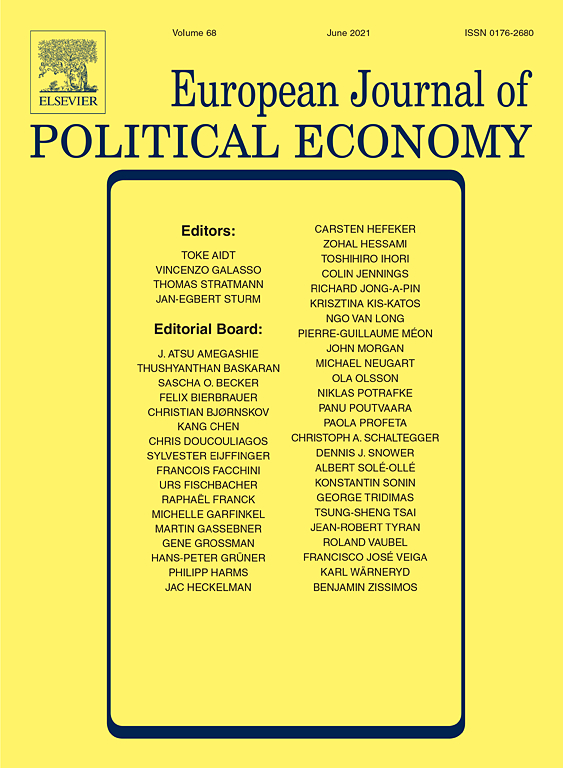
\includegraphics[scale=0.2]{/Users/hectorbahamonde/Job_Market/cover_ejpe.jpg}
		\end{figure}
	
	\end{columns}
\end{frame}


\miniframesoff
\begin{frame}\frametitle{``{\bf Still for Sale: The Micro-Dynamics of Vote Selling in the United States, Evidence From a List Experiment}.''}
	\begin{columns}
	\column{0.5\textwidth}
			\begin{itemize}
				\item {\color{ForestGreen}Democratic development and clientelism}.
				\item I designed a survey experiment (list experiment) and implemented it in \texttt{Qualtrics}.
				\item \emph{Original} data representative at the U.S. level.
				\item Acta Politica (forthcoming).
			\end{itemize}

	\column{0.5\textwidth}
		\begin{figure}[H]
		%\vspace{-2.5cm}
		\hspace{-7mm}
		
\includegraphics[scale=0.3]{/Users/hectorbahamonde/Job_Market/cover_ap.jpeg}
		\end{figure}
	\end{columns}
\end{frame}


\miniframesoff
\begin{frame}\frametitle{``{\bf Aiming Right at You: Group versus Individual Clientelistic Targeting in Brazil}.''}
	\begin{columns}
	\column{0.5\textwidth}
			\begin{itemize}
				\item {\color{ForestGreen}Inequality and clientelism}. 
				\item Observational data and matching methods for causal inference.
				\item Journal of Politics in Latin America (2018).
			\end{itemize}

	\column{0.5\textwidth}
		\begin{figure}[H]
		%\vspace{-2.5cm}
		\hspace{-7mm}
		
\includegraphics[scale=0.2]{/Users/hectorbahamonde/Job_Market/cover_jpla.png}
		\end{figure}
	\end{columns}
\end{frame}





\section{Research Plans}

\subsection{Pipeline summary}

\miniframesoff
\begin{frame}
\centering
\huge{My research plan at Turku is to continue studying these issues by moving forward several pieces of research I have in the pipeline.}
\end{frame}

% HERE


\miniframeson
\begin{frame}\frametitle{Pipeline 1: Clientelism}
\begin{enumerate} \setcounter{enumi}{0}
\item {\bf Lab and survey experiments}.
	\begin{itemize}
		\item ``{\input{/Users/hectorbahamonde/research/Economic_Experiment_Vote_Selling/title.txt}\unskip}'' ({\color{blue}{\input{/Users/hectorbahamonde/research/Economic_Experiment_Vote_Selling/status.txt}\unskip}}).
		
		\item ``{\input{/Users/hectorbahamonde/research/Conjoint_US/title_letter.txt}\unskip}'' ({\color{blue}{\input{/Users/hectorbahamonde/research/Conjoint_US/status_letter.txt}\unskip}}).
	\end{itemize}
\end{enumerate}
\end{frame}

\miniframesoff
\begin{frame}\frametitle{Pipeline 2: Inequality and COVID19}
\begin{enumerate} \setcounter{enumi}{1}
\item {\bf Natural experiments}.
	\begin{itemize}
		\item ``{\input{/Users/hectorbahamonde/research/Tobalaba/title.txt}\unskip}'' ({\color{blue}{\input{/Users/hectorbahamonde/research/Tobalaba/status.txt}\unskip}}).
		
		\item ``{\input{/Users/hectorbahamonde/research/Bus/title.txt}\unskip}'' ({\color{blue}{\input{/Users/hectorbahamonde/research/Bus/status.txt}\unskip}}).

	\end{itemize}
\end{enumerate}
\end{frame}

\subsection{Pipeline: survey and lab experiments}

\miniframeson
\begin{frame}\frametitle{{\scriptsize{``\input{/Users/hectorbahamonde/research/Economic_Experiment_Vote_Selling/title.txt}\unskip.}''}}
	%\begin{columns}
	%\column{0.5\textwidth}
		\begin{itemize}
			\item Economic experiment are ``games'': subjects embody randomly-assigned roles {\scriptsize(2 parties/1 voter)}.
			\item Study conditions under which ``parties'' buy and ``voters'' sell their votes contingent on randomly-assigned treatments:
			\begin{itemize}
				\item {\color{ForestGreen}Endowments}: ``parties'' and ``voters'' ({\color{blue}emulates income inequality}).
				\item {\color{ForestGreen}Ideology}: ideological distance between ``parties'' and ``voters.''
				\item {\color{ForestGreen}Contestation}: ``Risk'' of losing the election ({\color{blue}emulates party competition}).
			\end{itemize}
		\item {\bf Data are being collected as we speak} (N=200).
		\end{itemize}

	%\column{0.5\textwidth}
		%\begin{figure}[H]
		%\vspace{-2.5cm}
		%\hspace{-7mm}


		%\includegraphics[scale=0.5]{/Users/hectorbahamonde/research/Economic_Experiment_Vote_Selling/Experimental_Flow_Figure.pdf}
		%\end{figure}
	
	%\end{columns}
\end{frame}


\miniframeson
\begin{frame}\frametitle{{\scriptsize{``{\input{/Users/hectorbahamonde/research/Conjoint_US/title_letter.txt}\unskip}'' ({\color{blue}{\input{/Users/hectorbahamonde/research/Conjoint_US/status_letter.txt}\unskip}}).}}}		
\begin{itemize}
			\item I designed a conjoint experiment in \texttt{Qualtrics}.
			\item {\scriptsize{\bf Novel data} representative at the United States level (N=1,108).}
			\item {\bf Conjoint experiments} are good to study the causal effect of {\bf multiple-attribute treatments}.
			\item {\color{ForestGreen}Democratic theory}: Using Dahl's Polyarchy (1971), we devised different ``political candidates'' who supported different ``policies.''
			\item Tasked experimental subjects with choosing the ``lesser of two evils.''
			\item Using machine learning methods, we exploit that information to {\bf classify likely {\color{ForestGreen}vote-sellers}}.
\end{itemize}
\vspace{\fill}\hspace{\fill}\hyperlink{conjoint_table}{\beamerbutton{Example of experimental task}}
\end{frame}

\subsection{Pipeline 2: Inequality and COVID19}

\miniframeson
\begin{frame}\frametitle{{\scriptsize{``{\input{/Users/hectorbahamonde/research/Tobalaba/title.txt}\unskip}''.}}}		
\begin{itemize}
			\item Test
		\end{itemize}
\vspace{\fill}\hspace{\fill}\hyperlink{conjoint_table}{\beamerbutton{Example of experimental task}}
\end{frame}




\section{Last But Not Least}

\begin{frame}\frametitle{Last But Not Least}
\begin{itemize}
	\item Attending the main conferences in the discipline.
	\item Organizing a workshop/mini-conference per year at your institution.
	\item Giving service to the Philosophy, Contemporary History and Political Science Department, particularly, political science unit.
	\item Teaching and/or advising undergraduate/graduate courses/students.
	\item Assuming administrative tasks when necessary.
\end{itemize}
\end{frame}




\section{Appendix}

\subsection{Pipeline: Explained}


\miniframesoff
\begin{frame}\frametitle{{\scriptsize{``\input{/Users/hectorbahamonde/research/Economic_Experiment_Vote_Selling/title.txt}\unskip.}''}}
\begin{columns}

\column{0.5\textwidth}
{\bf Tell a supply and demand story}:
\begin{itemize}
	\item Do parties target own supporters {\scriptsize(Dixit/Londregan and Cox/McCubbins)} or moderate opposer {\scriptsize(Stokes)}? At what price?
	\item Under what conditions do vote sellers sell to their own party of choosing?
\end{itemize}

\column{0.5\textwidth}
	\begin{figure}[H]
		\vspace{-1cm}
		\hspace{-7mm}
		\includegraphics[scale=0.5]{/Users/hectorbahamonde/research/Economic_Experiment_Vote_Selling/Experimental_Flow_Figure.pdf}
	\end{figure}
\end{columns}
\end{frame}


\miniframesoff
\begin{frame}\frametitle{{\scriptsize{``{\input{/Users/hectorbahamonde/research/Conjoint_US/title_letter.txt}\unskip}'' ({\color{blue}{\input{/Users/hectorbahamonde/research/Conjoint_US/status_letter.txt}\unskip}}).}}\label{conjoint_table}}
	\begin{columns}\column{0.7\textwidth}
		\begin{itemize}
			\item {\color{ForestGreen}Democratic theory}: Dahl (1971) specifies a number of dimensions any ``polyarchy'' should accomplish (\emph{free press}, \emph{free competition}, \emph{right to run for elections}, etc.)
			\item The experiment captures in a causal way individual-level attitudes towards those dimensions. 
		\end{itemize}

	\column{0.3\textwidth}
\begin{table}[h]
\begin{center}
{\renewcommand{\arraystretch}{2}%
\scalebox{0.3}{
\hspace{-2cm}
\begin{tabular}{cc}
\hline
\multicolumn{1}{|c|}{{\bf Candidate 1}}   & \multicolumn{1}{c|}{{\bf Candidate 2}}  \\ \hline
\multicolumn{1}{|c|}{\small{Media CAN confront the government}}    & \multicolumn{1}{c|}{\small{Media CANNOT confront the government}}   \\ \hline
\multicolumn{1}{|c|}{\small{President CANNOT rule without Congress}}    & \multicolumn{1}{c|}{\small{President CAN rule without Congress}}   \\ \hline
\multicolumn{1}{|c|}{\small{Citizens CANNOT vote in the next two elections}}    & \multicolumn{1}{c|}{\small{Citizens CANNOT vote in the next two elections}}   \\ \hline
\multicolumn{1}{|c|}{\small{Citizens CAN run for office for the next two elections}}    & \multicolumn{1}{c|}{\small{Citizens CAN run for office for the next two elections}}   \\ \hline
\multicolumn{1}{|c|}{\small{Citizens CAN associate with others and form groups}}    & \multicolumn{1}{c|}{\small{Citizens CANNOT associate with others and form groups}}   \\ \hline
\multicolumn{2}{c}{\texttt{Which of these candidates represents the lesser of the two evils for you?}} \\ \hline
\multicolumn{1}{|c|}{\texttt{Candidate 1} {\large$\square$}} & \multicolumn{1}{c|}{\texttt{Candidate 2} {\large$\square$}} \\ \hline
\end{tabular}}
}
\end{center}
\end{table}
\end{columns}
\end{frame}


\miniframesoff
\begin{frame}\frametitle{{\scriptsize{``{\input{/Users/hectorbahamonde/research/Conjoint_US/title_letter.txt}\unskip}'' ({\color{blue}{\input{/Users/hectorbahamonde/research/Conjoint_US/status_letter.txt}\unskip}}).}}}
	\begin{columns}
	\column{0.5\textwidth}
		\begin{itemize}
			\item I also included a question about vote selling.
			\item This allows me to study which of those democratic dimensions specified by Dahl (1971) should fail to produce likely vote sellers.
			\item Finally, we use machine learning methods to {\bf classify likely {\color{ForestGreen}vote-sellers}}.
		\end{itemize}

	\column{0.5\textwidth}
		\begin{figure}[H]
		\vspace{-1cm}
		\hspace{-7mm}
		\includegraphics[scale=0.25]{/Users/hectorbahamonde/research/Conjoint_US/figure/w:analyses:p:p-1.pdf}
		\end{figure}
	
	\end{columns}
\end{frame}



\subsection{Abstracts}

% todos los papers, incluidos los publicados






\end{document}

